% !TeX root = paper-autotools-python.tex
% !TeX TXS-program:compile = txs:///pdflatex/[--shell-escape]
% https://orcid.org/0000-0003-4586-8500

\documentclass{article}
\usepackage{blindtext}

%%% FONTS %%%
\usepackage[T1]{fontenc}
\usepackage[utf8]{inputenc}
\usepackage[english]{babel}
%\usepackage{tgpagella} % set the document font to TeX Gyre Pagella
%\usepackage{tgbonum} % set the document font to TeX Gyre Bonum
%\usepackage{fontawesome5} % The Creative Commons icons

\usepackage{glossaries}

%%% DRAFT watermark %%%
\usepackage{draftwatermark}
\SetWatermarkText{DRAFT}
\SetWatermarkScale{5.1}
\SetWatermarkLightness{0.8}

\usepackage{xcolor} % \textcolor{red}{text} will be red for notes
\definecolor{lightgray}{gray}{0.6}
\definecolor{medgray}{gray}{0.4}

\usepackage{hyperref}
\hypersetup{
	colorlinks=true,
	urlcolor= blue,
	citecolor=blue,
	linkcolor= blue,
	% bookmarks=true,
	% bookmarksopen=false,
}

% for inserting images in line
\usepackage{graphicx}
\graphicspath{ {images} }

% Allows to rewrite the same title in the supplement
\newcommand{\mytitle}{Integration of GNU Autotools with Python Development Environments}
\usepackage{authblk}
\usepackage{comment} % allows block comments

\usepackage{ragged2e} % use flush and justify for text blocks
\usepackage{csquotes} % use \displayquote{} in the doc

%%% GRAPHICS  AND CODE BLOCKS %%%
\usepackage[listings, minted]{tcolorbox}
\usepackage{xcolor,colortbl}
\definecolor{myblue}{RGB}{0,163,243}
\definecolor{mygrey}{RGB}{128,128,128}
\definecolor{whitesmoke}{RGB}{245,245,245}
\newtcolorbox[auto counter, number within=section]{mybox}[2][]{
	colbacktitle=mygrey,
	colback=whitesmoke,
	title={#2},
	fonttitle=\ttfamily\small,
	fontupper=\sffamily\tiny,
	halign=flush left,
	rounded corners
}

%\usepackage[verbose]{wrapfig} % wrap text around image

\definecolor{myblue}{HTML}{4285F4} % color table cells

\usepackage[tablegrid]{vhistory} % version history package

% Headers and footers
\usepackage{fancyhdr}
\pagestyle{fancy}
\fancyhf{}
\lhead{Integration of GNU Autotools with Python Development Environments}
\lfoot{\tiny{June 03, 2022}}
\rfoot{\tiny{version: \vhCurrentVersion}}

% Code to add paragraph numbers and titles
\newif\ifptitle
\newif\ifpnumber
\newcounter{para}[section] % section x.y that resets in each new section
\newcommand\ptitle[1]{\par\refstepcounter{para}
	{\ifpnumber{\noindent\textcolor{lightgray}{\textbf{\thesection.\thepara}}\indent}\fi}
	{\ifptitle{\textbf{[{#1}]}}\fi}}
\ptitletrue  % comment this line to hide paragraph titles
\pnumbertrue  % comment this line to hide paragraph numbers


\begin{document}

\title{\mytitle}
\author[1,2]{Franklin E. Diaz\\ \texttt\href{emailto: fdiaz@paloaltonetworks.com}{fdiaz@paloaltonetworks.com}}
\affil[1]{Palo Alto Networks}
\affil[2]{Professional Services - Automation}
\begin{titlepage}
	\maketitle
\begin{abstract}
	The goal of this project paper is to detail my use of MIT Kerberos and OpenLDAP as an authentication mechanism for private cloud 
    computing environments. In addition to how the authentication mechanism is installed and configured, this paper will illustrate ways of
	using the mechanism to provision user accounts and show some examples of how the framework might be employed. The intent
	is to create an implementation that can be easily reproduced.
\end{abstract}
\end{titlepage}

\begin{comment}
Source files for this paper are available at: \url{https://github.com/devsecfranklin/paper-template/tree/main/}
\end{comment}


\section{\label{sec:Start}Integration of GNU Autotools with Python Development Environments}
\vspace{2mm}
\justifying
My effort to reduce the complexity and ease configuration issues when delivering Python heavy projects to customers and end
users has led to useful ways of working that I share in this paper. Autotools are a well-maintained set of Open Source tools
with a gentle learning curve and are included in the distribution of many Open Source packages that we all rely on daily, at
least indirectly. Here I have assembled certain battle-tested methods that I encourage others to understand and adopt.
\vspace{2mm}

\justifying
The list of tools for using this Autotools configuration paradigm is show in Table \ref{Autotools}.
\vspace{2mm}

\begin{table}[ht]
    \centering
    \begin{tabular}{|l|l|}\hline
        Tool & Description \\\hline
        autoconf & Generates a configure script from configure.ac   \\\hline
        automake & Generates a system-specific Makefile based on Makefile.am template    \\\hline
        make  &   X    \\\hline
    \end{tabular}
    \caption{Tools used in this project}
    \label{Autotools}
\end{table}
\vspace{2mm}


\justifying
In an effort to maintain a tidy development environment, the ``.gitignore'' file is appended with the following entries. These
entries will prevent intermediate build files from being checked in to revision control unnecessarily. Note that in the case
of ``aclocal'' it has been intentionally omitted since there is a sub-folder containing many m4 macros specific to Latex
document configuration and build.

\begin{mybox}[ht]{\thetcbcounter: Files to be excluded from revision control systems}
    \lstinputlisting{code/gitignore.txt}
\end{mybox}
\vspace{2mm}



\justifying
The image shown in Figure \ref{diagram} is from \cite{autobasics}.
The image illustrates the relationship between the components mentioned in Table \ref{Autotools}.
\vspace{2mm}

\begin{figure}[ht]
    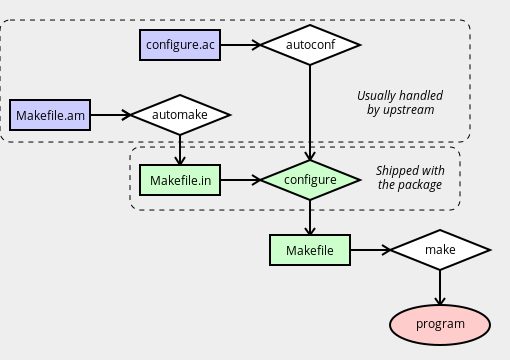
\includegraphics[width=12cm]{images/diagram.png}
    \caption{A basic overview of how the main autotools components fit together.}
    \label{diagram}
\end{figure}
\vspace{2mm}

\section{\label{sec:bootstrap}The bootstrap.sh script}

The purpose of the ``bootstrap.sh'' script is to allow project maintainers to prepare the local environment for use of autotools.
The boostrap script will attempt to guess if the local host is running a certain Linux distribution, or MacOS. There are execution
paths for each of these respective scenarios.

At first execution, autotools will run libtool, automake, and configure. Autotools creates a file named ``config.log''. If the config.log
file is found on subsequent runs of the script, fewer configuration steps will be performed since a certain system state is assumed. To
get a ``clean start'' the maintainer can simply delete the config.log file and rerun the bootstrap.sh script.

\justifying
A full working example of the bootstrap.sh script can be found in the source repository for this paper.

\begin{mybox}{\thetcbcounter: Steps to use Autotools}
    \lstinputlisting{code/steps.txt}
\end{mybox}
\vspace{2mm}

\section{\label{sec:config}The configure.ac file}
\vspace{2mm}
\justifying
A ``./configure'' script can be generated from a template named ``configure.ac''. This template is comprised of macros that are used to identify local system
software and program locations. In our case, we are interested in identifying the location of the Python 3.x installation on the local system.

\justifying
\href{https://www.gnu.org/software/automake/manual/html\_node/Python.html}{Per the automake documentation} we can define the minimum acceptable version of Python
and a variable that automake can use to refer to the version of Python discovered on the system. These declarative statements and the resultant values can then be
referenced by automake and added explicitly to the ``Makefile.am'' template.

\begin{mybox}{\thetcbcounter: Declaring Python Autoconf macros in configure.ac}
    \lstinputlisting{code/configure.ac}
\end{mybox}
\vspace{2mm}

\justifying
A full working example of the configure.ac file can be found in the source repository for this paper.

\section{\label{sec:make}The Makefile.am file}

\justifying
The ``Makefile.am'' file is a template that Automake uses to generate the full Makefile. Note that this project includes
``Makefile.am'' at the top level for setting up the Python virtual environment, and a second named ``paper/Makefile.am''
that contains directives on generating the PDF document you are reading now.

\begin{mybox}{\thetcbcounter: The Makefile.am for generating the top-level Makefile}
    \lstinputlisting{../Makefile.am}
\end{mybox}
\vspace{2mm}

\begin{mybox}{\thetcbcounter: The Makefile.am for generating the paper Makefile}
    \lstinputlisting{Makefile.am}
\end{mybox}
\vspace{2mm}

\section{\label{sec:req}Python requirements.txt files}

\justifying
My projects typically include three main requirements files, separated by functionality and named to foster a self-documenting paradigm.

\begin{table}[ht]
    \centering
    \begin{tabular}{|l|l|}\hline
        Filename & Description \\\hline
        src/requirements.txt & Common Python modules required by the main application.    \\\hline
        tests/requirements-test.txt & test, linting, syntax checking, formatting, etc.    \\\hline
        tests/requirements-security.txt  &  scan and secure the main app   \\\hline
    \end{tabular}
    \caption{Python requirements files}
    \label{Requirements}
\end{table}

\clearpage
\begin{versionhistory}
    \vhEntry{v0.1}{June 03, 2022}{Franklin Diaz}{Initial Draft}
\end{versionhistory}

\clearpage
% \nocite{*}
\bibliographystyle{plain}
\bibliography{mybib.bib}

\end{document}
